\documentclass{article}

% Language setting
% Replace `english' with e.g. `spanish' to change the document language
\usepackage[english]{babel}

% Set page size and margins
% Replace `letterpaper' with`a4paper' for UK/EU standard size
\usepackage[letterpaper,top=2cm,bottom=2cm,left=3cm,right=3cm,marginparwidth=1.75cm]{geometry}

% Useful packages
\usepackage{wrapfig}
\usepackage{graphicx}
\graphicspath{ {./images/} }
\usepackage{csquotes}
\usepackage[backend=biber]{biblatex}
\addbibresource{references.bib}

\title{Talos: A Beginner's Exploration of Avionics and Telemetry for Model Rockets}
\author{Nathan D. Alspaugh, Samuel J. Correa}

\begin{document}
\maketitle

\begin{abstract}
      In any aircraft or rocket, there are two systems present that are essential to any flight, the avionics and telemetry systems. The avionics system is responsible for controlling the flight path, monitoring the rocket's orientation, and collecting data. The telemetry system is responsible for transmitting this data to the ground station. In this paper, we present Talos, a project that aims to provide a beginner's perspective on the design and implementation of avionics and telemetry systems for model rockets. We document the process of learning to design and build Talos, from the initial planning phase to the final implementation and testing. We discuss the challenges faced, the lessons learned, and the future directions of the project. We hope that this paper will serve as a useful resource for students and hobbyists interested in exploring the field of avionics and telemetry for model rockets. Our results show that it is possible to design and build a functional avionics and telemetry system for model rockets using specialized components and open-source software that are accessible by any high school student. We believe that Talos has the potential to inspire others to explore the exciting world of aerospace engineering and rocketry.
\end{abstract}

\section{Introduction}

The avionics and telemetry systems are critical components of modern rocketry as they enable precise navigation, monitoring, and allow for the collection of data to later undergo optimizations. Being students with a passion for aerospace and mechanical engineering, we decided to explore these topics by building an avionics and telemetry system for model rockets. Talos, named after the mythical giant bronze automaton, is a project that aims to provide a beginner's perspective on the design and implementation of such systems. This paper documents the process of learning to design and build Talos, from the initial planning phase to the final implementation and testing.

\section{Background Research}

The term Avionics refers to the electronic systems used in aircraft and spacecraft. Avionics systems are responsible for navigation, communication, flight control, and monitoring. In the context of model rockets, avionics systems are used to control the flight path, collect data, and through telemetry, transmit to the ground station. This is made possible using a combination of Flight Control Systems, Air Data Systems, and Inertial Sensor Systems. Telemetry systems are used to transmit data from the rocket to the ground station using wireless communication protocols.


The Flight Control System employed in Talos is based on the auto stabilization (or stability augmentation) system described in \cite{Collinson_2012}. This system uses a combination of sensors to measure the rocket's orientation and adjust the control surfaces to maintain a desired flight path.


The Air Data System is responsible for measuring the rocket's altitude and airspeed. The system should compute these values from a combination of pressure and temperature sensors.

The Inertial Sensor System is used to measure the rocket's orientation and acceleration. This is achieved using sensors that can measure rotation (gyroscopes), sensors that can measure acceleration (accelerometers). In conjunction with the Air Data System, the INS can be used to compute the rocket's velocity vector information.

For the Telmetry System, we decided to use the LoRa (Long Range) protocol. LoRa is a long-range, low-power wireless communication protocol that is ideal for transmitting telemetry data from the rocket to the ground station. The LoRa protocol is based on spread spectrum modulation techniques, which increases reliability by "spreading" the signal over more frequencies, and is capable of transmitting data over long distances (up to 10 km) with low power consumption. This makes it ideal for use in model rockets, where power consumption and range are critical factors. It is also very immune to the doppler effects\cite{8723123} which is important for rockets that are moving at high speeds.

\section{Methodology}

The Talos project was divided into three main phases: Planning, Design, and Implementation. Each phase involved a series of tasks and challenges that needed to be addressed.

\subsection{Planning}

The planning phase involved defining the project scope, setting goals, and identifying the components needed. We started by researching existing avionics systems and telemetry solutions to understand the requirements and challenges involved. We then defined the key features of Talos, such as flight control, telemetry, and data logging. We also identified the components needed, such as sensors, microcontrollers, and communication modules.
\subsubsection{Breakout Board or Custom Printed Circuit Board (PCB)?}
After thorough research, we decided to create our own custom PCB for the Talos project. This was heavily impacted by the space constraints of the rocket, as well as the need for a powerful microcontroller with custom sensors that normal breakout boards (Arduino or ESP32) do not have. When we started the project, we had no experience with PCB design so we had to learn how to use EasyEDA, a free online PCB design tool.
\subsubsection{Microcontroller Selection}
We decided to use the STM32F405 microcontroller for the Talos project. This microcontroller has a powerful ARM Cortex-M4 core (180 mHz), plenty of I/O pins, and built-in support for various communication protocols. We chose this microcontroller because of its speed and versatility (see figure \ref{fig:microcontrollers}), as well as the availability of development tools and libraries. The STM32 Family has also been used in other aerospace applications, such as the CubeSat project \cite{Yost_2023}.
\begin{figure}[p]
      \caption{Table of STM32 Microcontrollers\cite{STM32_Table}}
      \label{fig:microcontrollers}
      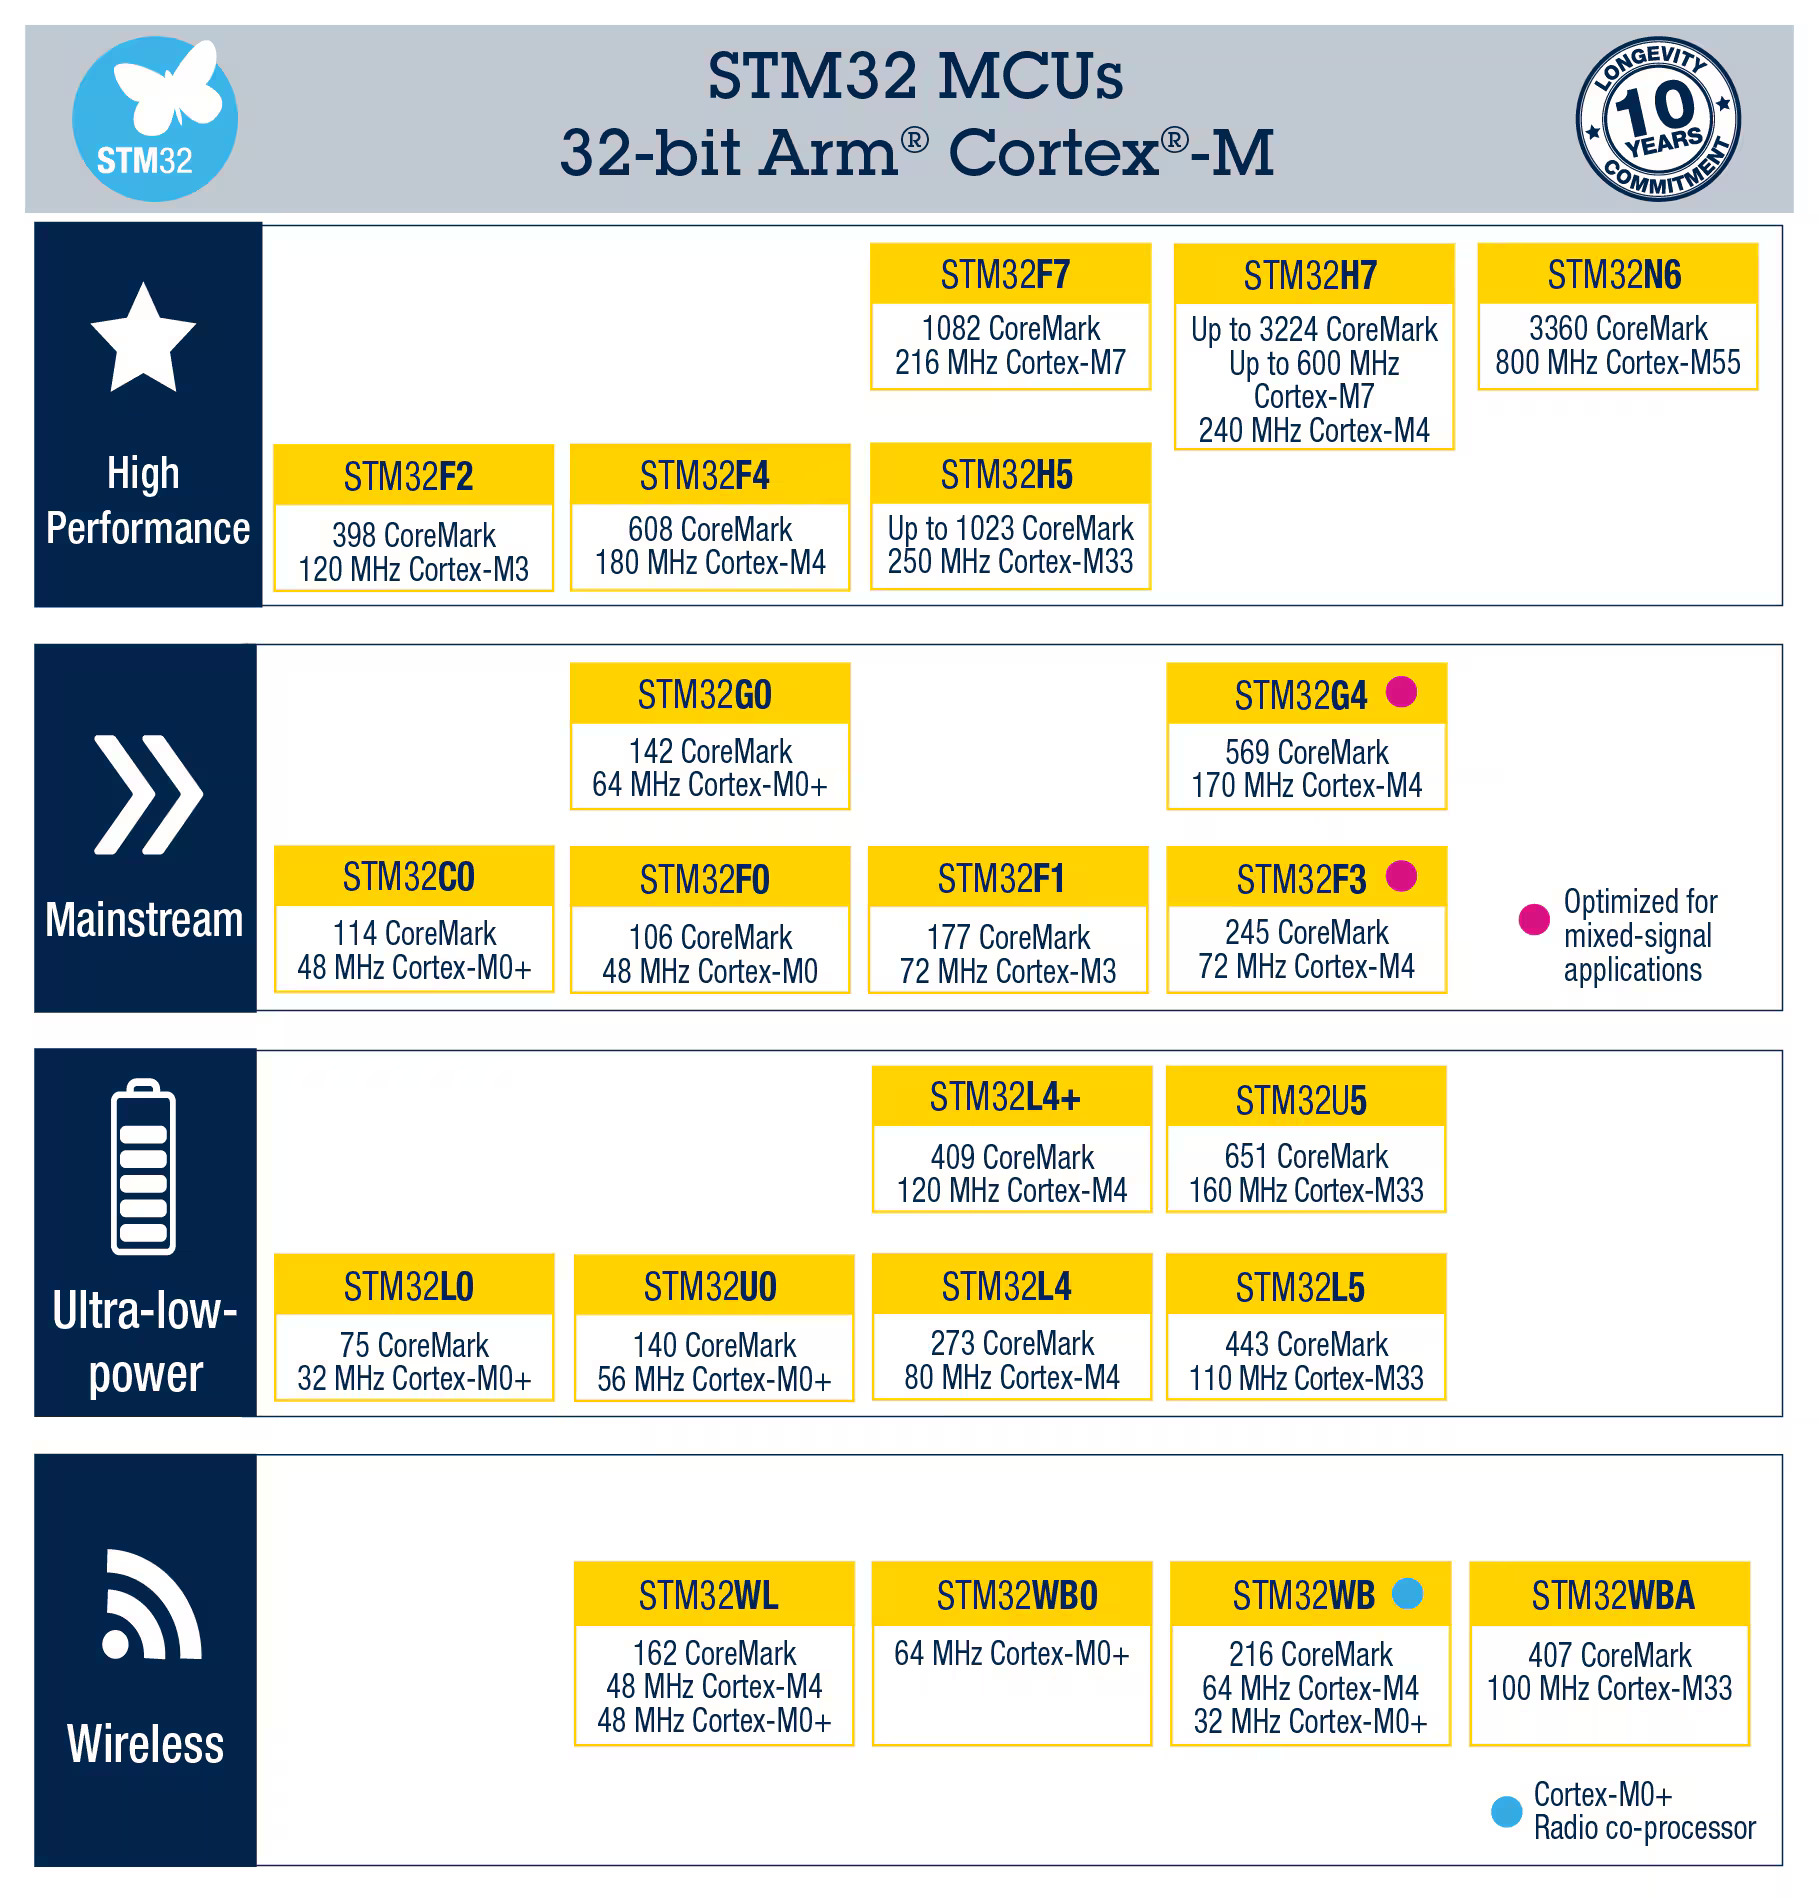
\includegraphics[width=\textwidth]{stm_mcu_chart.jpg}
      \centering
\end{figure}

\subsubsection{Sensor Selection}
\subsubsection*{Inertial Measurement Unit (IMU)}
We decided to utilize the LSM6DM IMU sensor for the Talos project. This sensor combines a 3-axis accelerometer and a 3-axis gyroscope in a single package. The LSM6DM is a MEMS (Microelectromechanical Sensor) capable of measuring acceleration and angular velocity in all three axes (see figure \ref{fig:lsm6dm}), making it ideal for measuring the rocket's orientation and acceleration. It also includes a thermometer to measure the temperature inside the rocket.
\begin{figure}[p]
      \caption{LSM6DM IMU Sensor\cite{LSM6DSM}}
      \label{fig:lsm6dm}
      \centering
      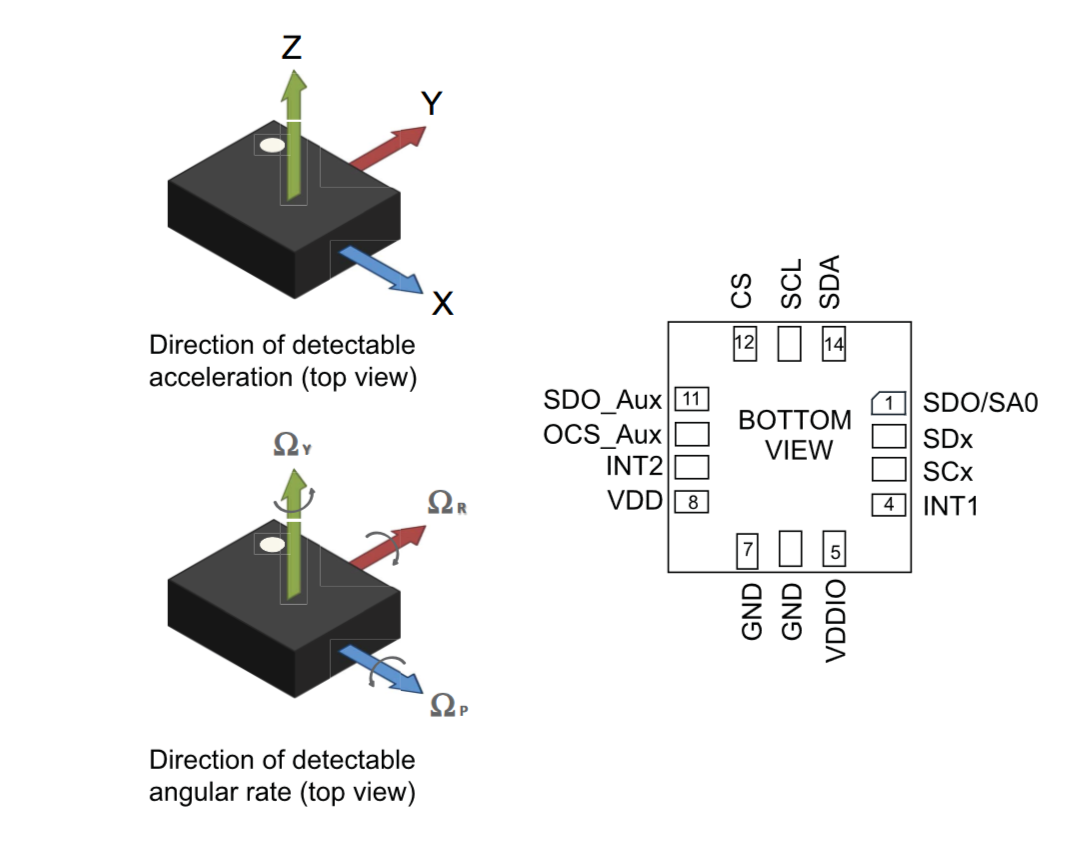
\includegraphics[width=\textwidth]{ldsm6m.png}
\end{figure}
\subsubsection*{Pressure Sensor}
\begin{figure}[p]
      \caption{BMP580 Pressure Sensor\cite{BMP580}}
      \label{fig:bmp580}
      \centering
      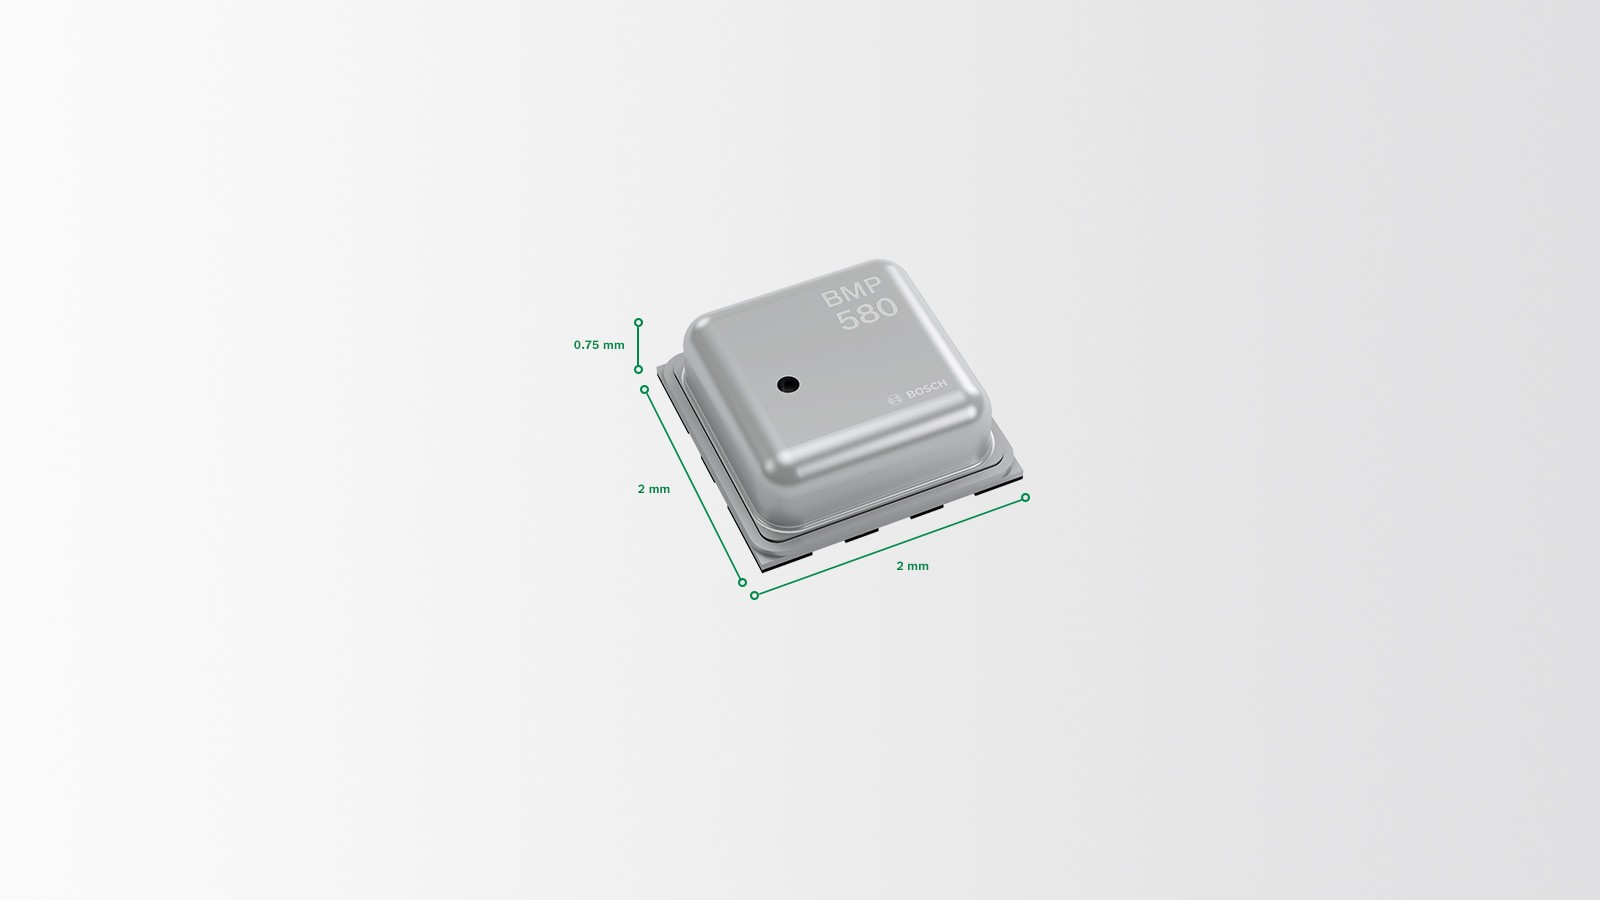
\includegraphics[width=\textwidth]{bmp580.jpg}
\end{figure}
For the pressure sensor, we decided to use the BMP580 (see figure \ref{fig:bmp580}). This sensor is capable of measuring pressure and temperature, which can be used to calculate the rocket's altitude and airspeed. It is also very accurate, more so than the more commonly used BMP280. \cite{Bosch_Sensortec_2024}

\subsubsection{Communication Module}
For the telemetry system, we decided to use the LLCC68 LoRa module and more specifically the DL-LLCC68-S-433 package. We use this package specifically because it transmits at 433 MHz, whose frequency is used for long range communication.

\subsection{Design}
After meticulously choosing parts, we decided to embark on the design phase. This phase involved creating the schematics and PCB layout for Talos. We started by designing the schematics in EasyEDA, which involved connecting the microcontroller, sensors, and communication modules. This was a huge challenge as we did not know how to connect each of the sensors. We had to learn how to read datasheets and understand the electrical characteristics of each component. Taking into account figure \ref{fig:lsm6dm}, we knew the basics of electronics, GND means ground, VDD means power, but the other pins were a complete mystery. Here are some terms that we had to learn:
\begin{itemize}
      \item Resistor: A resistor is a passive two-terminal electrical component that implements electrical resistance as a circuit element.
      \item Capacitor: A capacitor is a passive two-terminal electrical component that stores electrical energy in an electric field.
      \item Serial Peripheral Interface (SPI), a way to communicate between devices along a single data line. Imagine it like a bus, where each device is the stop and the data is the passengers. We select the stop using the Chip Select (CS) line and then send or recieve the date through the MOSI and MISO lines (SDO and SDA). The clock is used to synchronize the data and make sure that the bus arrives at the same time that the passengers are ready to board.
            \subitem SDO: Serial Data Out
            \subitem SDA: Serial Data In
            \subitem SCL: Serial Clock
            \subitem CS: Chip Select
      \item Inter-Integrated Circuit (I2C), a way to communicate between devices along a single data line. Using the same analogy as above with the bus but this time the driver doesn't know the directions of the stops and has to ask the passengers where to go. The SDA line is used to send and recieve data, while the SCL line is used to synchronize the data.
            \subitem SDA: Serial Data
            \subitem SCL: Serial Clock
      \item Interrupts, a way to notify the microcontroller that an event has occurred. This is like a bell that rings when the bus arrives at the stop.
      \item Universal Asynchronous Receiver-Transmitter (UART), a way to communicate between devices using two data lines. This is like a walkie-talkie, where one person talks and the other listens. The TX line is used to send data, while the RX line is used to recieve data.
      \item Pull-up and Pull-down resistors, resistors that are used to set the default state of a pin. Pull-up resistors are used to set the default state of a pin to high, while pull-down resistors are used to set the default state of a pin to low.
      \item Pull-up and Pull-down capacitors, capacitors that are used to filter out noise in a circuit. Pull-up capacitors are used to filter out noise in a high state, while pull-down capacitors are used to filter out noise in a low state.
      \item Decoupling capacitors, capacitors that are used to filter out noise in a circuit. These capacitors are used to filter out noise in the power supply.
\end{itemize}


\printbibliography

\end{document}